\documentclass{article}
\usepackage[brazil]{babel}
\usepackage[letterpaper,top=2cm,bottom=2cm,left=3cm,right=3cm,marginparwidth=1.75cm]{geometry}

\usepackage{amsmath}
\usepackage{graphicx}
\usepackage[colorlinks=true, allcolors=blue]{hyperref}

\title{Lista Especial de Problemas 12}
\author{Jeferson Almir}
\date{}

% 34

\begin{document}
\maketitle

\begin{enumerate}
    \item Um tabuleiro $10\times 10$ é particionado em 20 pentaminós
    por 80 segmentos unitários posicionados sobre arestas das casas.
    Qual é a quantidade máxima de diferentes pentaminós dentre esses 20?
    
    \item Um tabuleiro $7\times 14$ é construído de cópias do tetraminó de formato O e do triminó de formato V.
    É possível que:
    
    \begin{enumerate}
    \item a mesma quantidade de cópias de cada peça seja usada?
    
    \item mais cópias do tetraminó O sejam usadas que cópias do triminó V?
    \end{enumerate}
    
    \item Um $100$-minó pode ser decomposto em dois $50$-minós congruentes,
    ou então em $25$ tetraminós congruentes.
    É sempre possível decompó-lo em 50 dominós?
    
    \item Ana pinta várias casas de um tabuleiro $5\times5$.
    A tarefa de Bruno é cobrir todos eles
    colocando cópias de um triminó de formato V de forma que
    esses triminós não se sobreponham e cada triminó cubra exatamente 3 casas do tabuleiro.
    Qual é a quantidade mínima de casas que Ana deve pintar para garantir
    que Bruno não consiga completar sua tarefa?
    
    \item Uma casa no canto de um tabuleiro $8\times 8$ é pintada,
    e uma moeda é posta sobre ela.
    Pedro e Benício alternam turnos movendo a moeda, sendo Pedro o primeiro.
    Em seu turno, Pedro move a moeda uma vez como uma rainha do xadrez,
    parando numa casa não pintada.
    Benício em seu turno move a moeda duas vezes como um rei do xadrez,
    sempre indo para casas não pintadas.
    A casa visitada por Pedro e ambas as casas visitadas por Benício
    são então pintadas.
    O jogador sem movimentos possíveis perde o jogo.
    Qual jogador tem uma estratégia vencedora?
    
    \item Um poliminó é chamado de \textit{incrível}
    se ele não é retangular e várias cópias dele podem ser unidas para formar uma cópia maior dele.
    O diagrama a seguir mostra que o triminó V é incrível.
    
    \begin{center}
	    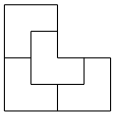
\includegraphics[scale=1]{img/img_12_01}
	\end{center}
	
	\begin{enumerate}
	\item Existe algum tetraminó incrível?
	
	\item Determine todos os $n>4$ tais que
	existe um $n$-minó incrível.
	\end{enumerate}
	
	\item Numa caixa $7\times 7$,
	cada um dos 49 chocolates é preto ou branco.
	A cada movimento, Alex pode comer dois chocolates adjacentes por uma linha,
	por uma coluna ou por uma diagona, dado que eles sejam do mesmo tipo.
	
	Qual é a quantidade máxima de chocolates que Alex pode garantir
	poder comer, independentemente da disposição inicial dos chocolates?
	
	\item Uma espaçonave alienígena invisível no formato de um tetraminó O
	pode pousar num campo $7\times 7$,
	ocupando 4 dos 49 quadrados unitários.
	Sensores podem ser postos em alguns desses quadrados.
	Um sensor vai enviar um sinal se está num quadrado no qual a espaçonave pousou.
	Da localização de todos os sensores que mandarem sinal, devemos ser capazes de
	determinar exatamente em quais quatro quadrados a espaçonave pousou.
	Qual é a menor quantidade de sensores que devemos posicionar?
	
	\item Bento tem uma quantidade suficientemente grande de cópias do tricubo I,
	que é um bloco $1\times1\times3$,
	e do tricubo V, que é um bloco $1\times2\times2$ com um cubo unitário faltando.
	Bento constrói com essas peças uma caixa sólida retangular
	onde cada dimensão é no mínimo 2.
	Qual é quantidade mínima de cópias do tricubo I que Bento deve usar?
\end{enumerate}

\end{document}